\section{系统功能与展示}
\label{sec:showcase}

\begin{figure}[t]
	\centering
	\subfloat[概览]{
		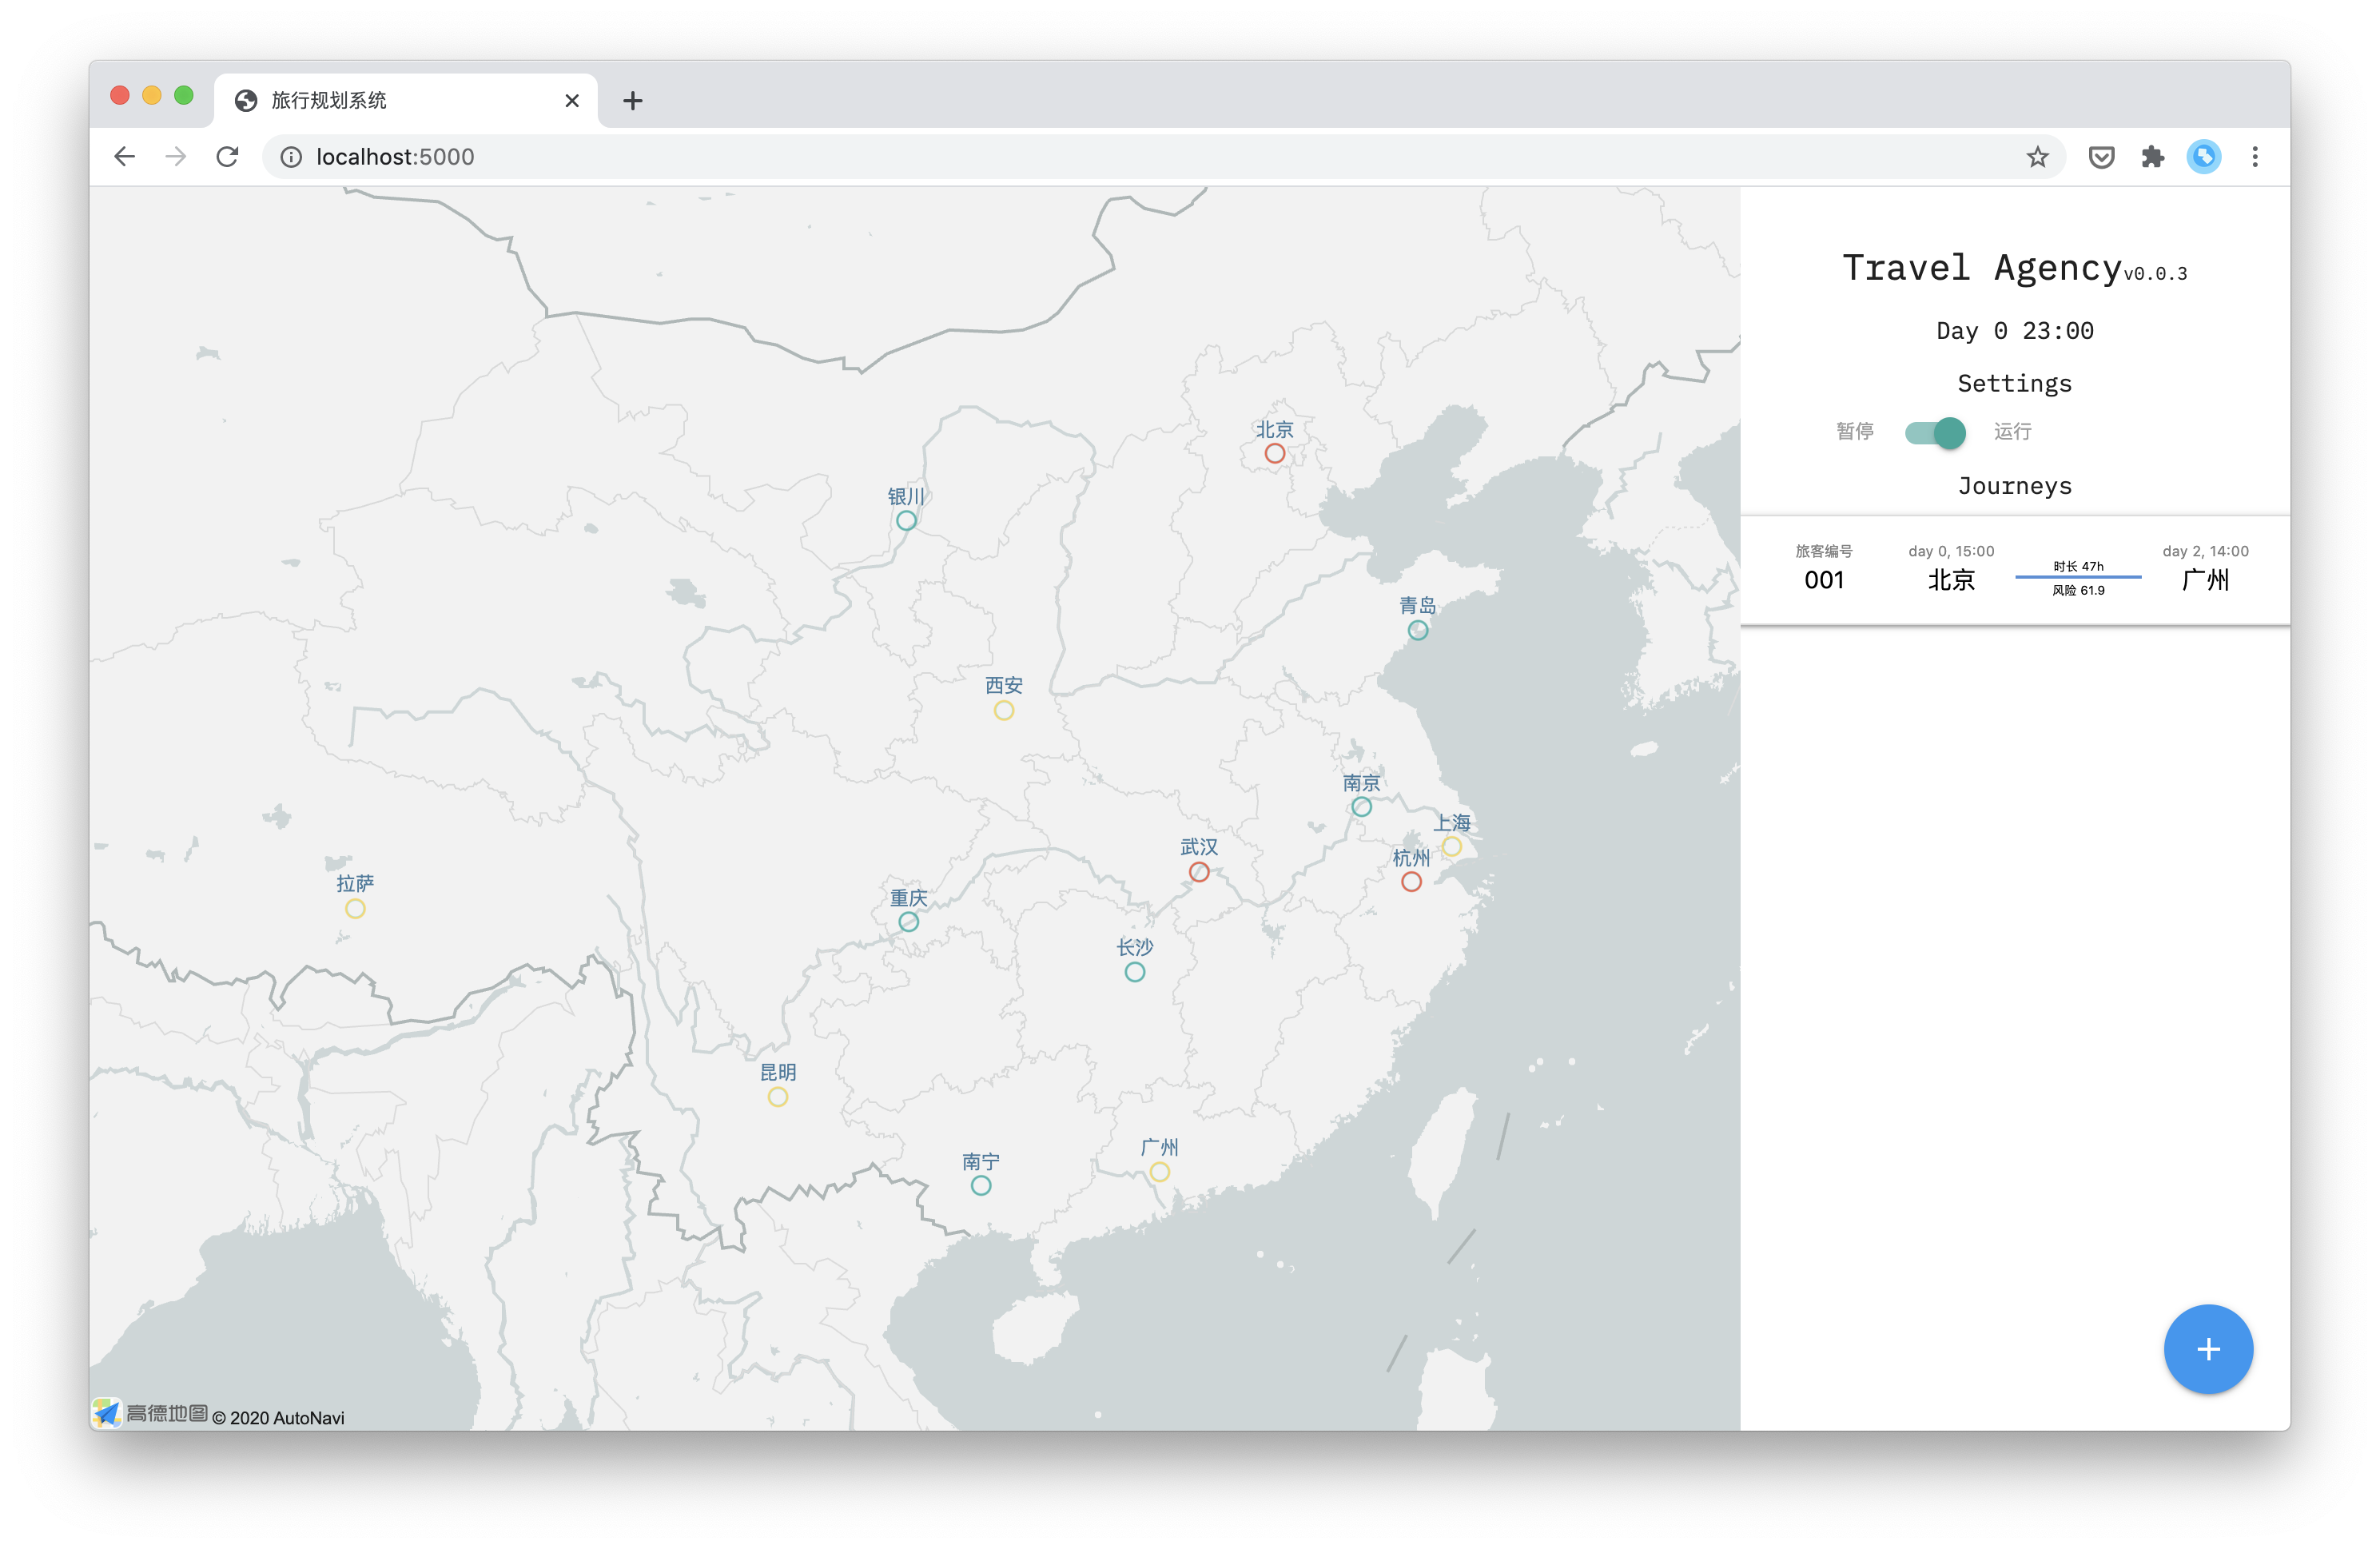
\includegraphics[width=0.5\textwidth]{figures/screenshot_overview}
		\label{fig:showcase-overview}
	}
	\subfloat[旅程状态]{
		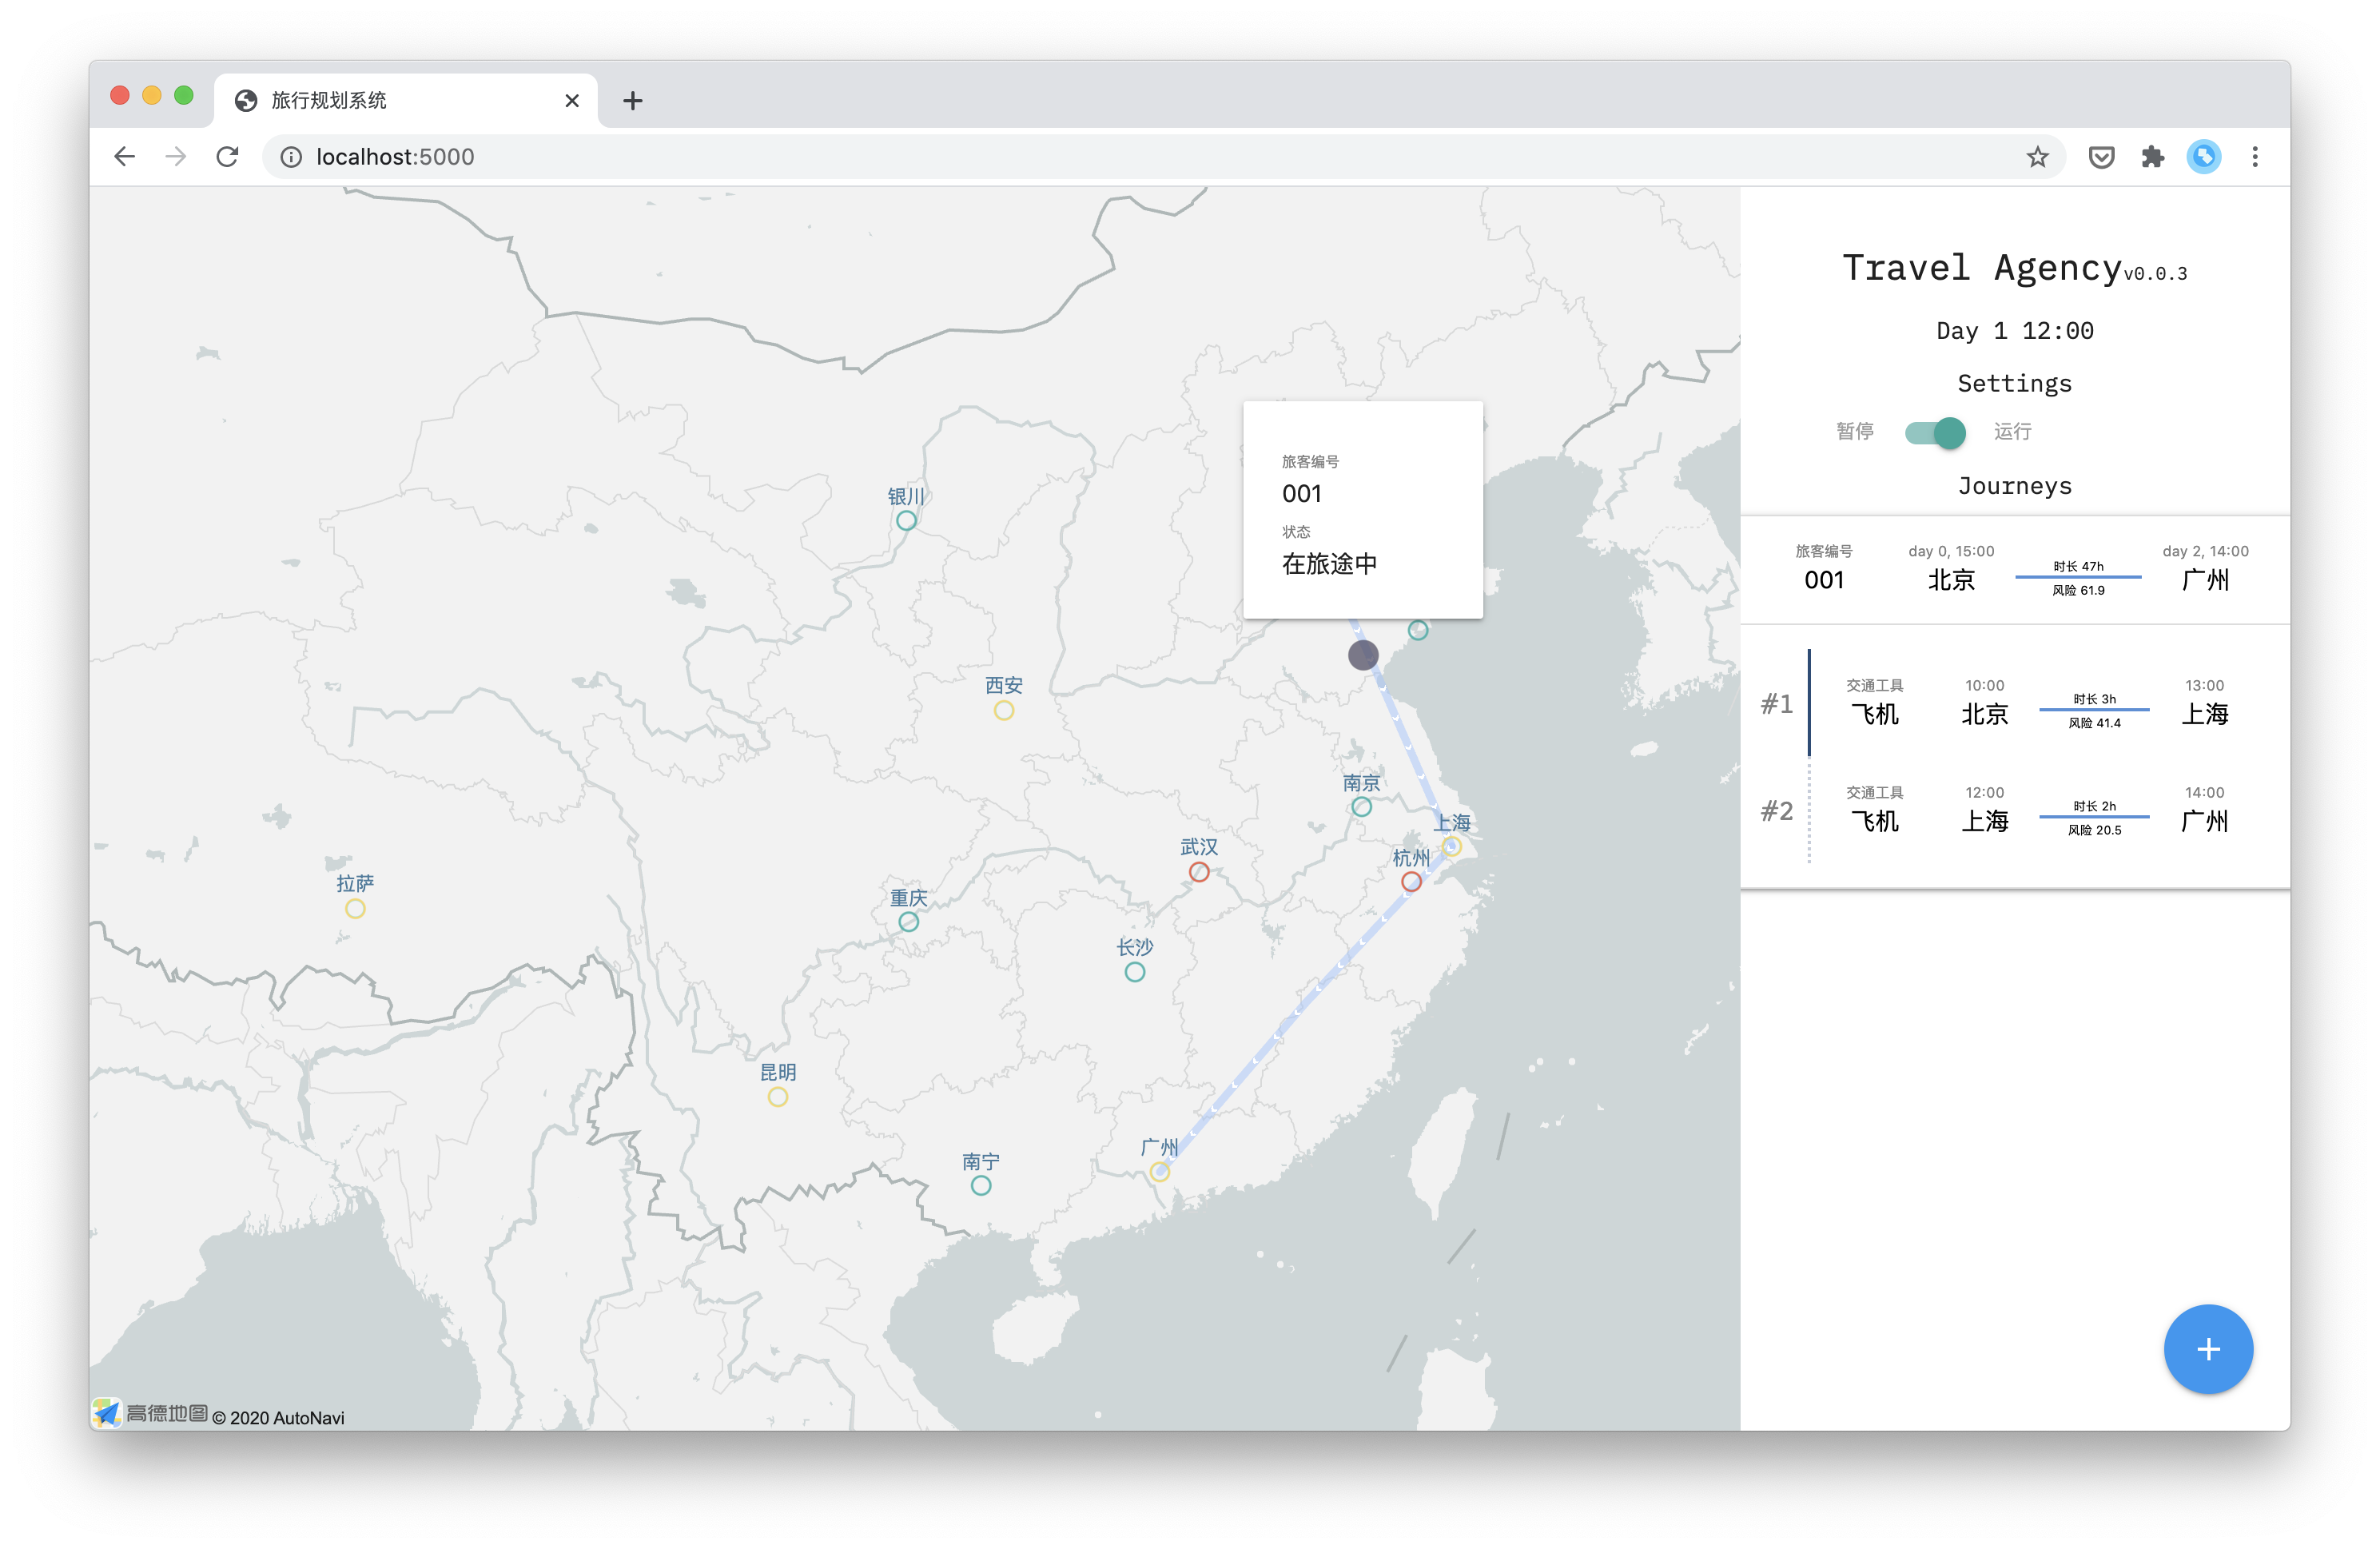
\includegraphics[width=0.5\linewidth]{figures/screenshot_journey_details}
		\label{fig:showcase-journey-details}
	}
	\caption{系统界面概览}
	\label{fig:showcase}
\end{figure}

本小节将简单地展示\textsc{TravelAgency}系统,并且概述系统功能。

\subsection{系统界面}

图 \ref{fig:showcase} 展示了\textsc{TravelAgency}系统的界面。可以看到系统界面分为两个部分。

\begin{enumerate}[(a)]
  \item 地图。显示城市信息,也能实时显示旅途信息。对于旅途信息,会绘制旅途中搭乘的线路,以及旅客当前所在位置。将鼠标移到旅客图标上,会给出旅客号、当前状态等更加具体的信息。如图 \ref{fig:showcase-journey-details} 中所示。
  \item 信息面板。信息面板中包含了各类信息,包括:当前时间,当前进行中的旅程。点击旅程列表中的某一旅程,将显示出旅程的详细信息,包括每一步搭乘的线路、每一步所花费的时间、带来的旅程风险等等。同时,信息面板中也包含控制系统暂停运行的按钮,以及添加旅程的按钮(右下角加号按钮)。
\end{enumerate}

\begin{figure}[t]
	\centering
	\subfloat[添加旅程]{
		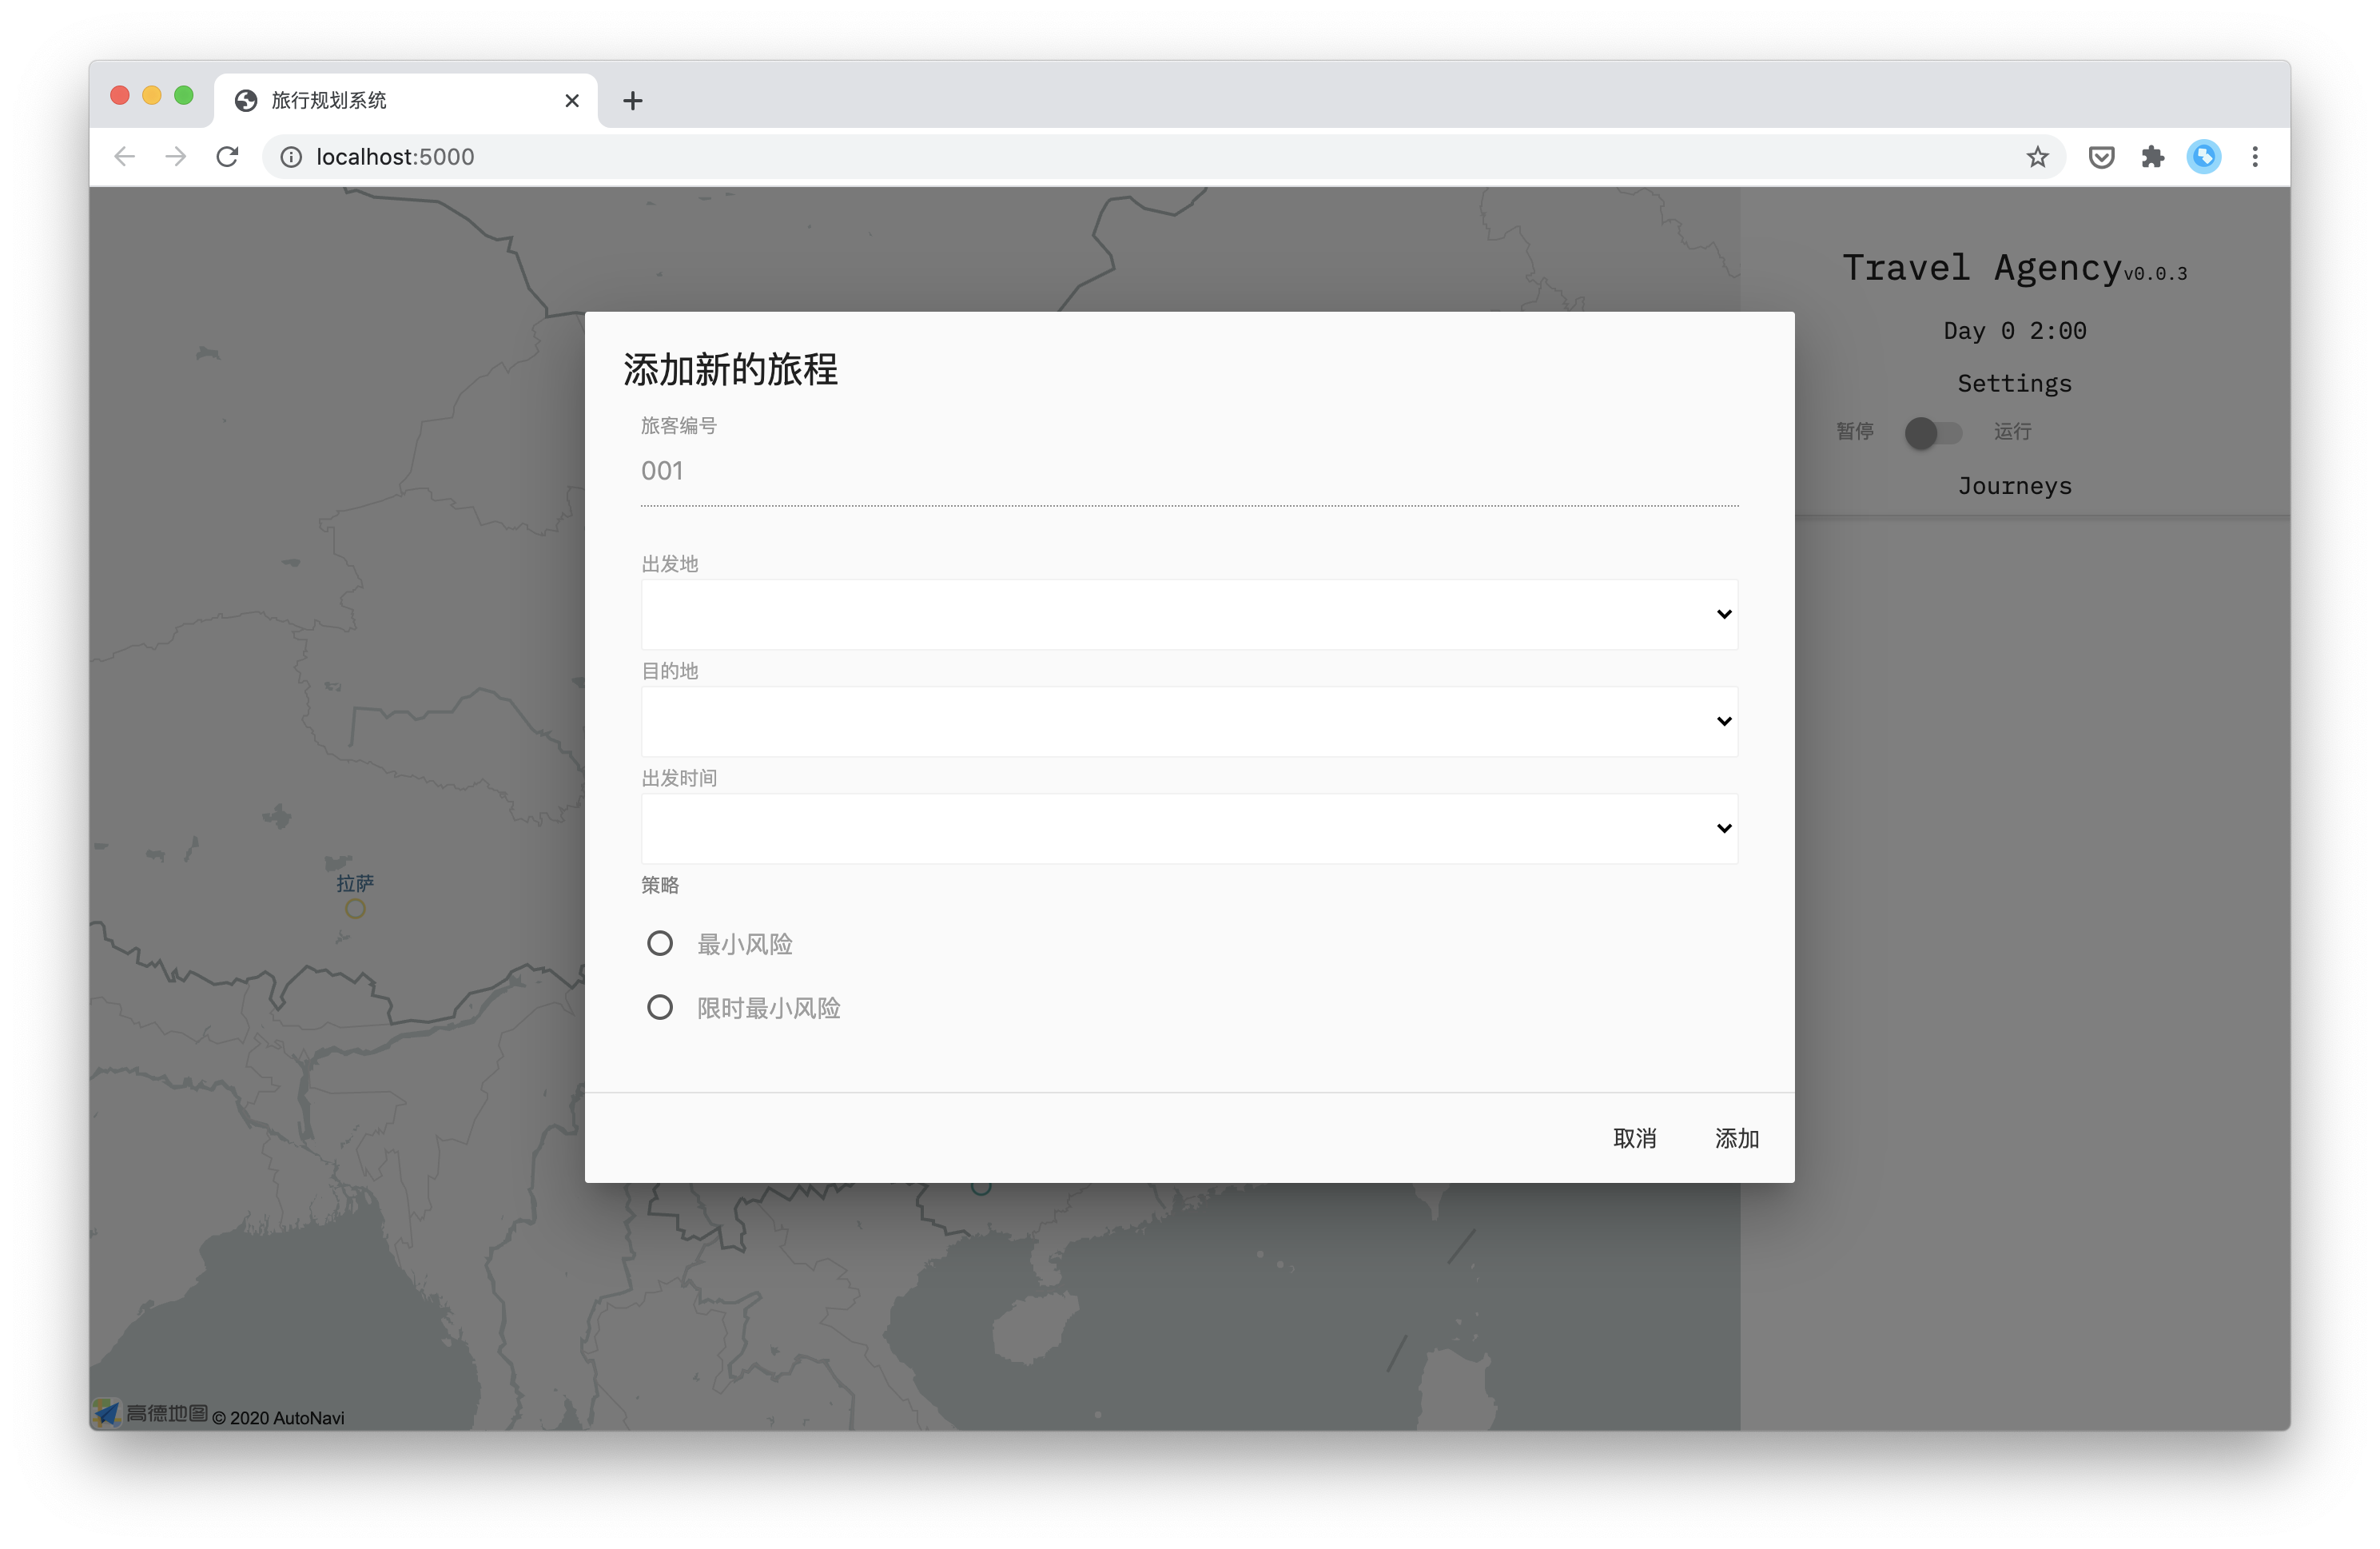
\includegraphics[width=0.5\textwidth]{figures/screenshot_add_journey}
		\label{fig:showcase-add-journey}
	}
	\subfloat[预览旅程信息]{
		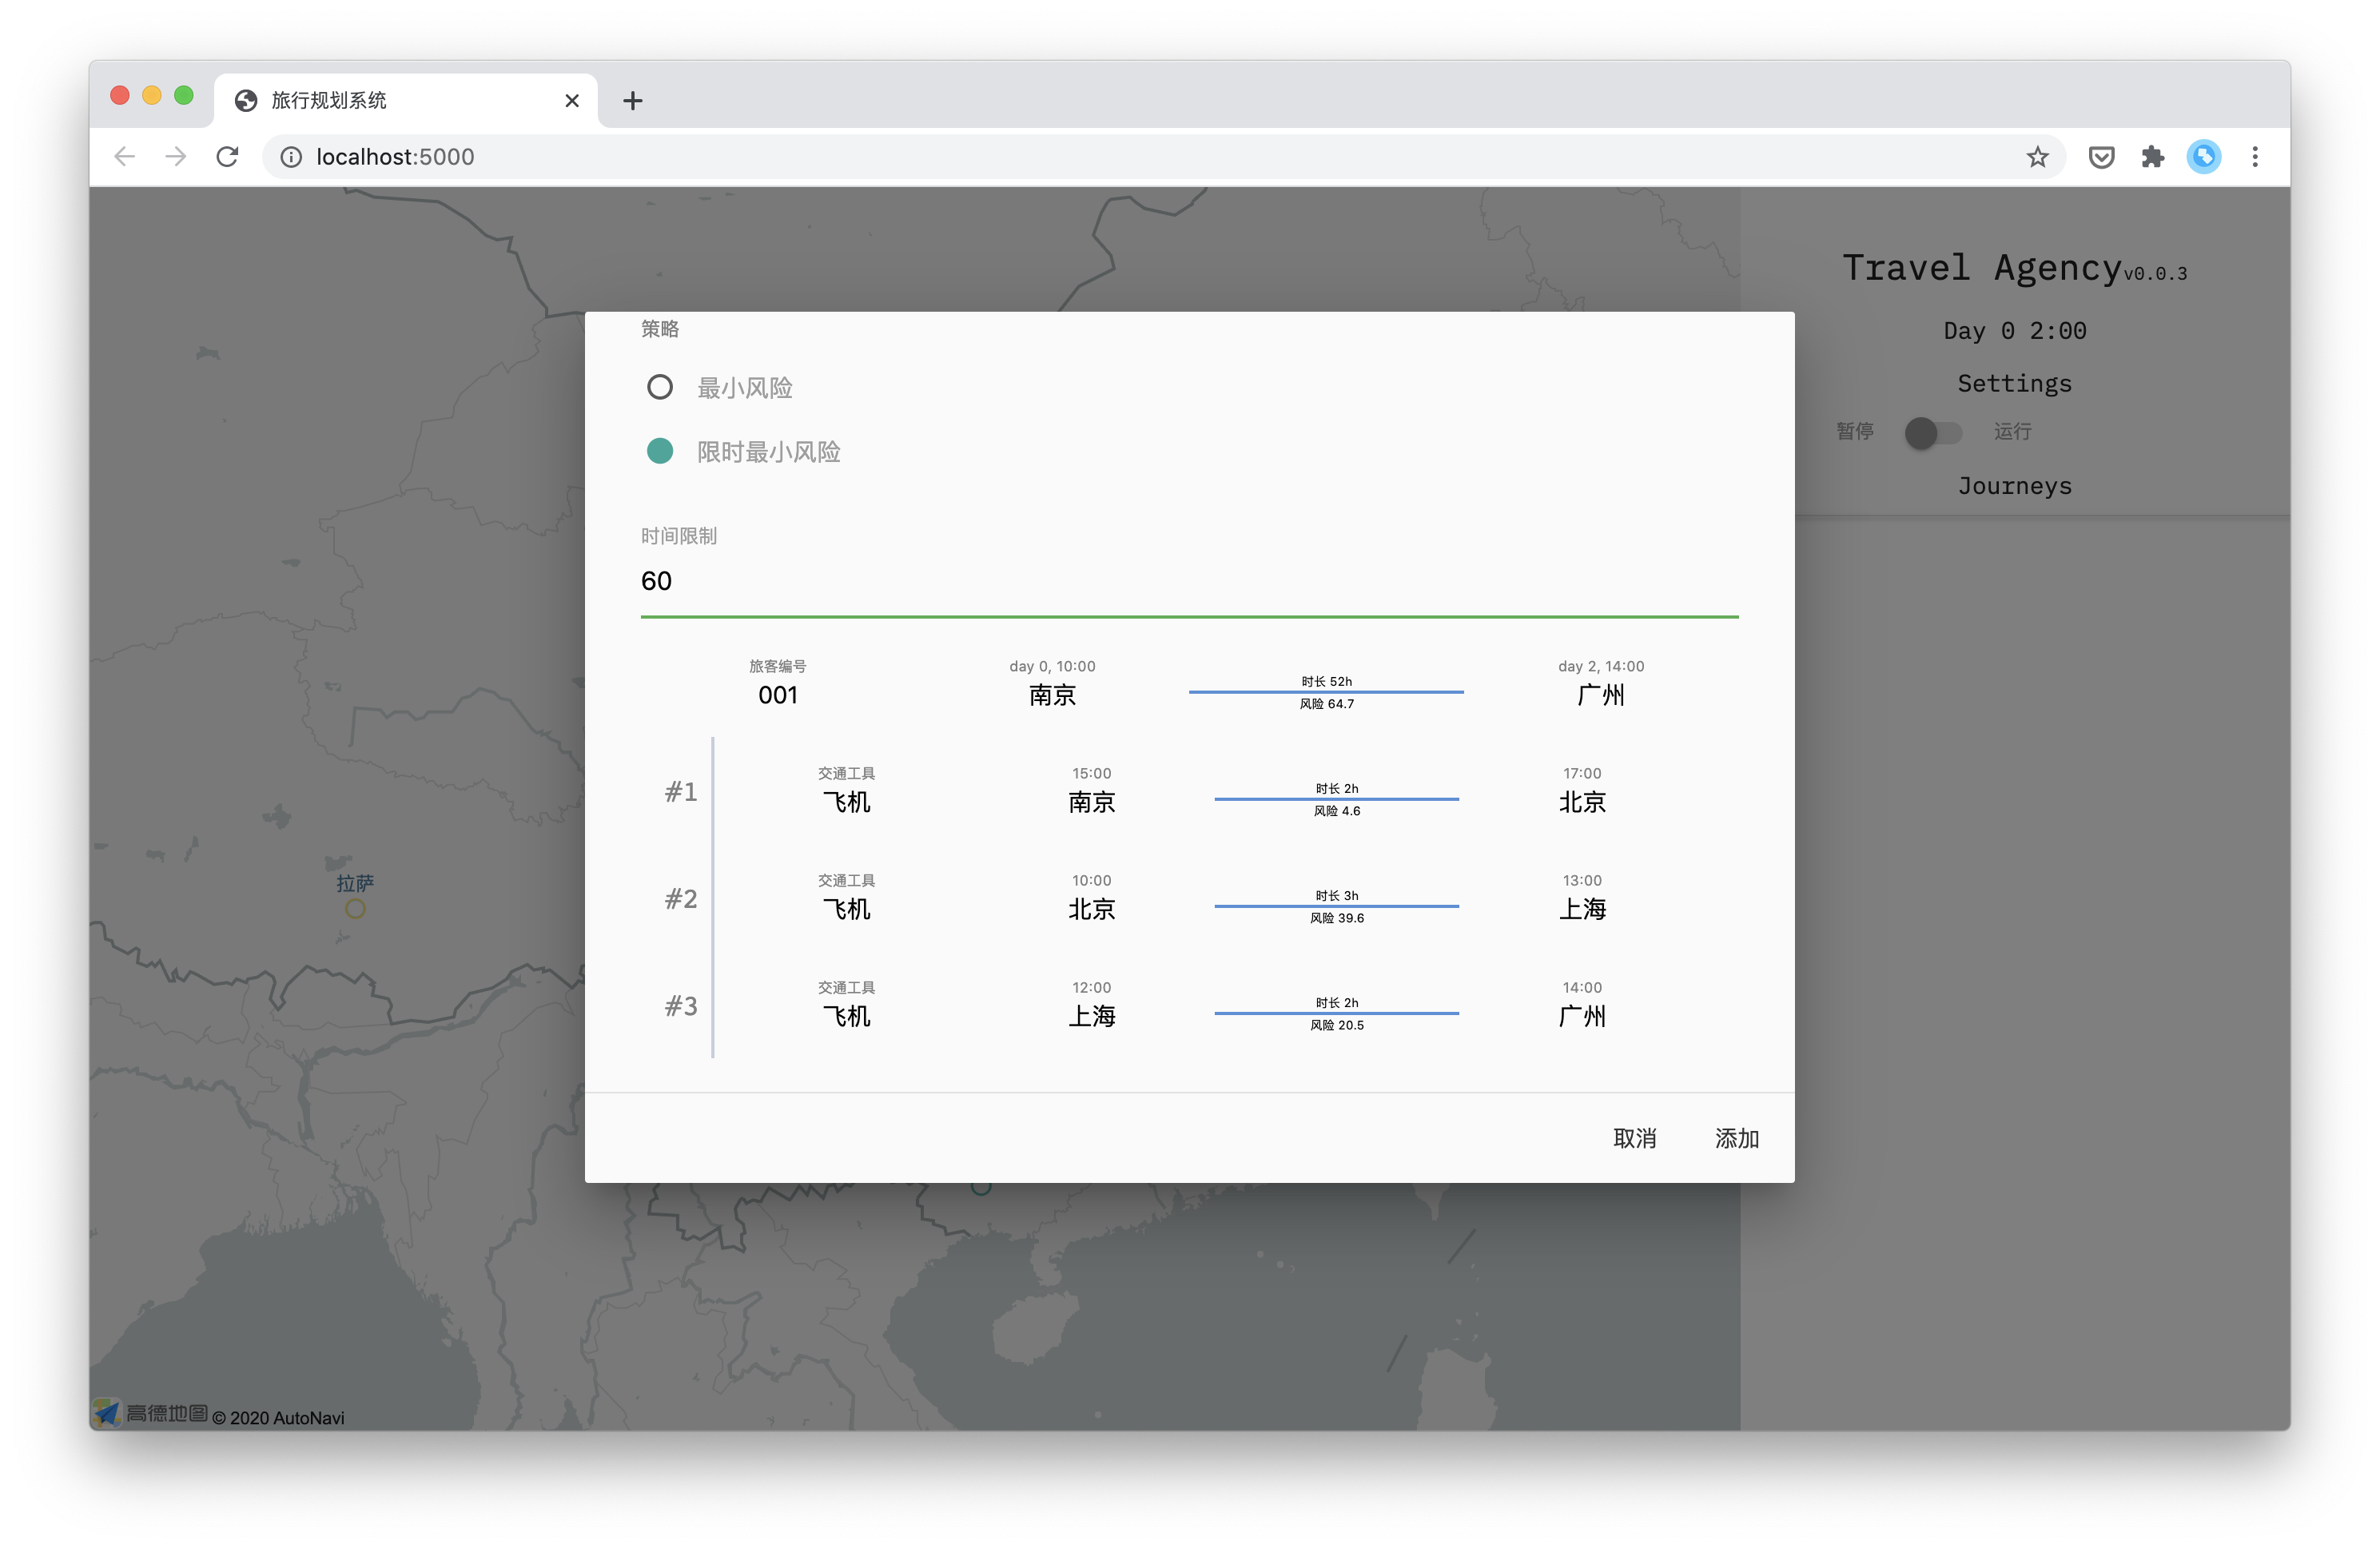
\includegraphics[width=0.5\linewidth]{figures/screenshot_add_journey_preview}
		\label{fig:showcase-add-journey-preview}
	}
	\caption{添加旅程界面}
	\label{fig:showcase-2}
\end{figure}

而图 \ref{fig:showcase-2} 中展示了在点击添加旅程的按钮之后,弹出的添加旅程界面。在这一见面中,需要输入新旅程的各类信息:出发地点、目的地点、出发时间、旅行策略,若旅行策略为限时最小风险策略,还需要输入时间限制。如图 \ref{fig:showcase-add-journey-preview} 中所示。

在输入完旅程信息之后,系统能够自动加载规划出的旅行方案,如图 \ref{fig:showcase-add-journey-preview} 中所示。旅行方案包含总时间、总风险,以及每一步的详细信息等。在确认无误之后,点击添加,就能将旅程添加到系统中。若对信息进行修改,在修改完成后,系统会自动更新显示修改后的旅行方案。点击取消,就能取消添加新的旅行。

注意到,在添加旅行的过程中,系统时间自动处于暂停状态。在取消添加或者确认添加之后,系统时间会自动恢复运行。

\subsection{系统主要功能}

系统包含以下主要功能:

\definecolor{high-risk}{HTML}{ED553B}
\definecolor{mid-risk}{HTML}{F6D55C}
\definecolor{low-risk}{HTML}{3CAEA3}

\begin{enumerate}[(a)]
  \item \textbf{显示城市地图}。如图 \ref{fig:showcase-overview} 中所示,系统能够将城市显示在地图上。用不同颜色的圈来表示不同的风险等级。具体地,\textit{{\color{high-risk}红色}}代表高风险地区;\textit{{\color{mid-risk}黄色}}代表中风险地区;\textit{{\color{low-risk}绿色}}代表低风险地区。
  \item \textbf{两种策略的低风险旅行规划}。\textsc{TravelAgency}能够实现最小风险、限时最小风险策略的旅行规划。\textit{且不仅能考虑到等待带来的风险,也能够考虑到旅程中的风险}。
  \item \textbf{实时显示旅行状态}。系统能够实时显示旅行的状态。能够将旅行线路绘制在地图上,并且显示旅客所处位置与状态,如:等待出发,在旅途中,正在等候,已抵达。且能直观、美观地显示出每条旅程的详细信息。
  \item \textbf{暂停、继续系统时间}。系统能够自由地暂停、继续时间运行。当添加旅行时,系统时间自动停止。
\end{enumerate}








